\chapter[Méthodologie]{Méthodologie}
\label{Methodologie}

\chapterabstract
{Plusieurs plateformes et algorithmes du Datamining ont été employés dans la littérature scientifique pour estimer la visibilité, comme c'est déjà mentionné dans le chapitre introductif. Pour effectuer notre étude, nous avons choisi 
 5 plateformes open source (\textit{Scikit-learn}, \textit{H2O}, \textit{WEKA}, \textit{Tensorflow} et \textit{Keras}) et 4 algorithmes Datamining (\textit{Random Forest}, \textit{Gradient Boosting Machine}, \textit{eXtreme Gradient Boosting} et \textit{Deep Learning}).
Ce chapitre, est dédié  à la méthodologie adoptée pour atteindre les objectifs du stage. Ainsi, nous présenterons au début les plateformes open source, les bibliothèques et les packages utilisés. Par la suite, nous expliquerons le principe de chaque algorithme et ses spécifications, et nous terminerons par les configurations expérimentales adoptées pour le développement des modèles, ainsi que les outils de diagnostics pour évaluer leur performance.}
\pagestyle{plain}

%%%%%%%%%%%%%%%%%%%%%%%%%%%%%%%%%%%%%%%%%%%%%%%%%%%%%%%%%%%%%%%%%%%%%%%%%%%%%%%%%%%%%%%%%%%%%%%%%%%%%%%%%%
\section{Plateformes open sources utilisées}\label{plref}
%%%%%%%%%%%%%%%%%%%%%%%%%%%%%%%%%%%%%%%%%%%%%%%%%%%%%%%%%%%%%%%%%%%%%%%%%%%%%%%%%%%%%%%%%%%%%%%%%%%%%%%%%%
\subsection{WEKA}\label{defWeka}
\begin{wrapfigure}{l}{0.2\textwidth}
    
\includegraphics[width=0.2\textwidth]{img/wekalogo.png}
\end{wrapfigure}
\textit{WEKA} \footnote{disponible sur le web: www.cs.waikato.ac.nz/ml/weka} (Waikato Environment for Knowledge Analysis) est une plateforme open source développée sous Java, qui offre un ensemble d’outils permettant de traiter et d’analyser des fichiers de données. Une collection des algorithmes d'apprentissage automatique (machine learning) est disponible dans cette plateforme. Elle a été développée à l'Université de Waikato en Nouvelle-Zélande \citep{witten2016data}. \\

Sa version originale a été développée en 1992 à la base d'un mélange entre Tk/Tcl\footnote{Tool Command Language/Tool Kit Tool Command Language.}, du langage C et de Makefile\footnote{C'est un fichier contenant un ensemble de directives utilisé par un outil d'automatisation de compilation pour générer une cible / un objectif.}. En 1997, la décision fut prise de développer une nouvelle fois \textit{WEKA} à partir de zéro en Java, y compris l'implémentation des algorithmes de modélisation. En 2005, \textit{WEKA} reçoit le prix SIGKDD (Data Mining and Knowledge
Discovery Service Award). Une année après, en 2006, Pentaho\footnote{est une solution d'informatique décisionnelle open source entièrement développée en Java.} acquiert une licence exclusive pour utiliser \textit{WEKA} dans sa suite décisionnelle open source (version communautaire et
commerciale).  \\


En plus de l'implémentation d'une large gamme d’algorithmes Datamining, plusieurs avantages distingue cet outil dont nous citons quelques-uns:
\begin{itemize}
\item[\textbullet] \textit{WEKA} est disponible en source libre et est gratuit sous la licence GNU\footnote{C'est une licence qui fixe les conditions légales de distribution d'un logiciel libre du projet GNU.};
\item[\textbullet] Portable car il est entièrement implémenté en Java et donc fonctionne sur quasiment toutes les plateformes modernes, ainsi, que tous les systèmes d'exploitation actuels;
\item[\textbullet] \textit{WEKA} contient une collection complète d'outils de prétraitement de données et de techniques de modélisation ;
\item[\textbullet] Facile à utiliser en raison de l'interface graphique qu'il offre.
\item[\textbullet] \textit{WEKA} supporte plusieurs outils d'exploration de données standards, en particulier des prétraiteurs de données, \textit{clustering} de données, des classificateurs statistiques, des analyseurs de régression, des outils de visualisation, et des outils d'analyse discriminante.
\end{itemize}
Cependant, ce logiciel a certain limites en termes de manipulation des analyses complexe et ainsi de visualisation,
\begin{itemize}
\item[\textbullet] \textit{WEKA} n'est pas capable de faire de l'exploration de données multi-relationnelles ;
\item[\textbullet] Certaines fonctionnalités de cette plateforme ne sont pas facilement manipulables comparativement à un logiciel concurrent. 
\item[\textbullet] \textit{WEKA} GUI (Graphical User Interface) fournit plusieurs panneaux intégrés de 'visualisation', mais ceux-ci sont très limités, car la visualisation en \textit{WEKA} se concentre sur la compréhension du comportement des algorithmes, plutôt que sur les ensembles de données ;
\item[\textbullet] L’interface graphique n’est pas aussi bien documentée ou intuitive.
\end{itemize}


\subsection{H2O} \label{defH2O}
\begin{wrapfigure}{l}{0.1\textwidth}
    
\includegraphics[width=0.1\textwidth]{img/h2ologo.png}
\end{wrapfigure}
\textit{H2O} est une plateforme open source d'apprentissage automatique distribuée en mémoire. Elle est produite par la société H2O.ai\footnote{C'est une société spécialisée dans le domaine d’intelligence artificielle et du machine learning.}. Cette plateforme est dédiée à effectuer des analyses prédictives en utilisant des algorithmes de Machine Learning. Elle prend en charge les algorithmes du statistique et d’apprentissage automatique les plus largement utilisés, notamment \textit{Gradient Boosting Machine}, les modèles linéaires généralisés, \textit{Random Forest}, \textit{eXtreme Gradient Boosting}, \textit{Deep learning}, etc.\\

La société H2O.ai a été lancé en 2011 à Mountain View, en Californie (dans la Silicon Valley). La société s'appelait à l'origine 0xdata, mais elle a changé de nom en 2014 pour correspondre à son produit phare, H2O. La plateforme \textit{H2O} est utilisée par plus de 18 000 organisations dans le monde et est extrêmement populaire dans les communautés R et Python.\\


Les principaux avantages de la plateforme \textit{H2O}: 
\begin{itemize}
\item[\textbullet] \textit{Rapide}, tant à l’installation, qu’à la prise en main que dans ses performances algorithmiques.
\item[\textbullet] \textit{Scalable} (évolutif), offre la possibilité d’exploiter un cluster hadoop\footnote{C'est un framework open source qui repose sur Java il prend en charge le traitement des données volumineuses (Big Data) au sein d'environnements informatiques distribués.} existant ou de monter un cluster h2o dédié.
\item[\textbullet] \textit{H2O} est basé sur java et propose une gestion optimisée de la mémoire. 
\item[\textbullet] manipulable via l’interface web fournie ou via des connecteurs pour les langages d’analyse les plus populaires (R, Python, Java, Scala, Spark)\\
\end{itemize}

Les deux limites de cette plateforme les plus répandues sont:   
\begin{itemize}
\item[\textbullet] \textit{H2O} sous Windows ne supporte pas l'algorithme \textit{xGBoost}.
\item[\textbullet] \textit{H2O} étant une plateforme en mémoire, la taille des données est largement limitée par taille de RAM dont vous disposez. 
\end{itemize}


\subsection{Scikit-learn}\label{defscikit}
\begin{wrapfigure}{l}{0.2\textwidth}
    
\includegraphics[width=0.2\textwidth]{img/scikitlogo.png}
\end{wrapfigure}
\textit{Scikit-learn} est un module Python open source sous BSD License\footnote{Berkeley Software Distribution License} (distribution des logiciels de Berkeley), intégrant une large gamme d’algorithmes d’apprentissage automatique qu'ils soient supervisés et non supervisés. Ce paquet met l'accent sur l'apprentissage automatique aux non-spécialistes utilisant un langage de haut niveau. L'accent est mis sur la facilité d'utilisation, les performances, la documentation et la cohérence des API\footnote{Application Programming Interface} (Interface Applicative de Programmation). Ce qui encourage son utilisation dans les milieux académiques et commerciaux \citep{pedregosa2011scikit}. \\


\textit{Scikit-learn} est un code collaboratif à la base, initié par David Cournapeau (promo 2004 Télécom ParisTech\footnote{C'est une grande école d’ingénieurs publique française, spécialisée dans le domaine des technologies de l'information de la communication.}) en 2006. Et comme un sujet du doctorat de Matthieu Brucher ainsi qu'il a été soutenu par plusieurs autres “Google Summer Code”, et par l'Inria (Institut national de recherche en informatique et en automatique) à partir de 2010.\\

Les API de base ont été définies et une liaison efficace de LibSVM \citep{chang2011libsvm} confère au projet un avantage concurrentiel. En décembre 2011, le premier sprint international a été organisé avec un financement généreux de Google. Aujourd'hui, le projet a largement dépassé l'INRIA pour devenir une plateforme mondiale ouverte \citep{article}.\\

Ce qui distingue cette plateforme est sa popularité, en effet il compte plus de 1308 contributeurs à la date de réalisation de cette étude répartis dans le monde, notamment aux États-Unis et en Australie, et on estime à plus de 300 000, le nombre d’utilisateurs réguliers. Le papier historique publié en 2011 a quant à lui dépassé les 16449 citations dans google scholar. Enfin, \textit{Scikit-learn} est largement diffusé dans le milieu académique (à l’école comme dans les plus grandes universités mondiales, la librairie logicielle est utilisée dans les enseignements de machine learning) et industriel (voir les témoignages de Spotify, Change.org ou encore DataRobot sur le site).\\

Outre sa popularité cet outil est se caractérisée par autres avantages nous citons:
\begin{itemize}
\item[\textbullet] \textit{Scikit-learn} simples et efficaces pour l'exploration et l'analyse de données ;
\item[\textbullet] Accessible à tous et réutilisable dans divers contextes ;
\item[\textbullet] Construit sur NumPy\footnote{C'est une bibliothèque Python, qui prend en charge de grands tableaux multidimensionnels et matrices, ainsi qu’une vaste collection de fonctions mathématiques de haut niveau.}, SciPy\footnote{C'est un projet visant à unifier et fédérer un ensemble de bibliothèques Python à usage scientifique. Scipy utilise les tableaux et matrices du module NumPy.} et matplotlib\footnote{C'est une bibliothèque Python destinée à tracer et visualiser des données sous formes de graphiques.} ;
\item[\textbullet] Open source, utilisable dans le commerce - Licence BSD.\\
\end{itemize}

En d'autre part, nous mentionnons quelques limitations de cette plateforme, comparativement aux concurrents dans le même domaine:
\begin{itemize}
\item[\textbullet] Il ne supporte pas le GPU (Processeur graphique) \footnote{Graphics Processing Unit};
\item[\textbullet] Destiné à l'apprentissage machine, plus que l'apprentissage en profondeur (i.e. Deep learning).
\end{itemize}


\subsection{TensorFlow}\label{defTensor}
\begin{wrapfigure}{l}{0.2\textwidth}
    
\includegraphics[width=0.2\textwidth]{img/tensorlogo.png}
\end{wrapfigure}
\textit{Tensorflow} est une puissante bibliothèque d’apprentissage automatique orientée flux de données (Data flow) créée par l'équipe Google Brain de Google et rendue open source en 2015. Elle est conçue pour être facile à utiliser et largement applicable à la fois pour de problèmes liés aux réseaux numériques et neuronaux, ainsi que d'autres domaines. \textit{Tensorflow} est l'un des outils les plus utilisés en intelligence artificielle dans le domaine de l'apprentissage automatique \citep{wiki:xxx}.\\

Le projet Google Brain\footnote{C'est une équipe de recherche en Deep learning et en intelligence artificielle travaillant chez Google. Formé au début des années 2010, Google Brain associe des recherches ouvertes sur l'apprentissage automatique avec ingénierie des systèmes et des ressources informatiques à l'échelle de Google.} a débuté en 2011 pour explorer les utilisations de réseaux de neurones profonds à très grande échelle, à la fois pour la recherche et pour une utilisation dans les produits de Google. Dans le cadre des premiers travaux de ce projet, l'équipe de Google Brain a construit DistBelief, la première génération évolutive d'apprentissage. Et grâce à l'expérience d'équipe avec DistBelief et d'une compréhension plus complète des propriétés de système souhaitables et des exigences en matière d'apprentissage et d'utilisation de réseaux neuronaux, \textit{Tensorflow} a connu le 11 février 2017, la naissance de la deuxième génération de système Google Brain pour la mise en œuvre et le déploiement de modèles d'apprentissage automatique à grande échelle. En février 2018, Google a annoncé la mise à disposition de TPUs\footnote{Tensor Processing Unit.} (unité de traitement de tenseur) en version bêta sur la plateforme Google Cloud \citep{girija2016tensorflow}.\\


Ce qui encourage les utilisateurs de cette outil est ses avantages représenté ci-dessous:
\begin{itemize}
\item[\textbullet] Open source rapide, flexible, et évolutif pour la recherche et la production ;
\item[\textbullet] Portabilité : \textit{Tensorflow} s'exécute sur des GPUs, CPUs (Unité centrale de traitement)\footnote{ Central Processing Unit } et TPUs, desktops et sur les serveurs. Ainsi, il donne la possibilité de déployer un modèle entraîné sur un mobile en tant que partie de produit, et c'est ainsi qu'il constitue une véritable fonctionnalité de portabilité \citep{softwebsolutions}.
\item[\textbullet] \textit{Tensorflow} disponible pour plusieurs langages : Python, R, C++, Java, C\# etc ;
\end{itemize}



\subsection{Keras}\label{defKeras}
\begin{wrapfigure}{l}{0.2\textwidth}
    
\includegraphics[width=0.2\textwidth]{img/keraslogo.png}
\end{wrapfigure}
\textit{Keras} est une API de réseaux de neurones de haut niveau, écrite en Python. En effet, c'est un framework d’apprentissage en profondeur (deep learning) qui offre un moyen pratique de définir et de former presque tous les types de modèles d’apprentissage en profondeur. \textit{Keras} a été initialement développé pour les chercheurs, dans le but de permettre une expérimentation rapide. Ainsi, il est capable de s'exécuter sur \textit{Tensorflow}, Microsoft Cognitive Toolkit (CNTK) ou Theano \citep{Chollet2018}.\\

\textit{Keras} compte plus de 250 000 utilisateurs individuels à la moitié du 2018 (d'après la documentation de cet outil), allant des chercheurs universitaires aux ingénieurs des startups et des grandes entreprises aux étudiants diplômés et aux amateurs. \textit{Keras} est utilisé chez Google, Netflix, Uber, CERN, Yelp, Square et des centaines de startups travaillant sur un large éventail de problèmes. C'est également un framework populaire sur Kaggle\footnote{le site Web du concours d’apprentissage automatique}, où presque tous les concours récents d’apprentissage en profondeur ont été gagnés avec des modèles \textit{Keras}.\\


Il a été développé dans le cadre des efforts de recherche du projet ONEIROS\footnote{Open-ended Neuro-Electronic Intelligent Robot Operating System.} (Système d’exploitation de robot intelligent neuroélectronique). Son auteur et responsable principal est François Chollet, un ingénieur de Google. Sa première publication a eu lieu le 27 mars 2015.\\

En 2017, l'équipe \textit{Tensorflow} de Google a décidé de prendre en charge \textit{Keras} dans la bibliothèque principale de \textit{Tensorflow}. Puis Microsoft a également ajouté à \textit{Keras} un backend CNTK, disponible à partir de CNTK v2.0.\\

De ce qui suit, nous résumons les avantages de cet API dans les points suivants: 
\begin{itemize}
\item[\textbullet] Open source ;
\item[\textbullet] Permet un prototypage simple et rapide (convivialité, modularité et extensibilité) ;
\item[\textbullet] Prend en charge les réseaux convolutifs et les réseaux récurrents, ainsi que les combinaisons des deux ;
\item[\textbullet] Fonctionne parfaitement sur CPU et GPU ;
\item[\textbullet] \textit{Keras} avait plusieurs backends tels que \textit{Tensorflow}, \textit{CNTK} et \textit{Theano} ;
\item[\textbullet] \textit{Keras} est compatible avec Python.\\
\end{itemize}


Cependant, \textit{Keras} ne gère que les API de haut niveau qui s'exécutent sur un autre moteur ou infrastructure tels que \textit{Tensorflow}, \textit{Theano} ou \textit{CNTK}.\\


Les cinq plateformes, packages et bibliothèques expliqué précédemment sont des outils open-source que nous avons utilisé au cours de ce travail, leurs configurations et la comparaison entre elles sera expliqué respectivement dans le chapitre modélisation \ref{conf_plat} et le chapitre évaluation \ref{comp_plat}. \\

Dans la section suivante, nous allons décrire les principaux algorithmes que nous avons adopté pour cette étude, leur principe, leur spécificité et quelques principaux hyperparamètres propres à chacun d'entre eux. 



%%%%%%%%%%%%%%%%%%%%%%%%%%%%%%%%%%%%%%%%%%%%%%%%%%%%%%%%%%%%%%%%%%%%%%%%%%%%%%%%%%%%%%%%%%%%%%%%%%%
\newpage
\section{Algorithmes Datamining utilisés}\label{algo_used}
%%%%%%%%%%%%%%%%%%%%%%%%%%%%%%%%%%%%%%%%%%%%%%%%%%%%%%%%%%%%%%%%%%%%%%%%%%%%%%%%%%%%%%%%%%%%%%%%%%%
Dans cette section, nous allons décrire brièvement les algorithmes d'apprentissage supervisé adoptés en mettant en exergue les spécificités de chacun. Ainsi, deux grandes classes purement distinctes ont été utilisées :
\begin{itemize}
    \item[\ding{224}] Les algorithmes issus des méthodes ensemblistes basées sur l'agrégation des modèles;
    \item[\ding{224}] L'apprentissage profond (deep learning).
\end{itemize}

Les algorithmes issus des méthodes ensemblistes sont basés sur des stratégies adaptatives (boosting, gradient boosting) ou aléatoires (bagging, random forest) permettant d’améliorer l’ajustement par une combinaison
ou agrégation d’un grand nombre de modèles tout en évitant ou contrôlant le sur-ajustement. \\

Remis en veilleuse depuis le milieu des années 90 au profit d’autres algorithmes  d’apprentissage  machine ou  plutôt  statistique : boosting,  random forest..., les réseaux de neurones connaissent un regain d’intérêt et même un énorme battage médiatique sous l’appellation d’apprentissage profond (deep learning). 

\subsection{Random Forest}
\textit{Random Forest} (RF) \citep{breiman2001random} est un algorithme d'apprentissage automatique de famille des modèles ensemblistes (\textit{Ensemble Methods}) qui suit la technique du \textit{Bagging} \footnote{Bagging est une abréviation de Bootstrap aggregating, sert à faire un échantillonnage de données en des sous ensembles.} \citep{breiman1996bagging} améliorée par l'ajout d'une composante aléatoire. L’objectif est donc de rendre plus indépendants les arbres de l’agrégation en ajoutant du hasard dans le choix des variables qui interviennent dans les modèles. Ses estimateurs de base sont des arbres de décision. Il se charge de sélectionner de manière aléatoire un ensemble d’entités \textit{features} qui sont utilisées pour déterminer la meilleure répartition au niveau de chaque nœud de l’arbre de décision \citep{wang2016estimation}.\\

En termes simples, et vu que nous traitons un cas de régression, \textit{Random Forest} combine un grand ensemble d'arbres de régression, chaque arbre représente un ensemble de conditions ou de restrictions organisées hiérarchiquement et appliquées successivement du racine à la feuille de l'arbre, comme indiqué dans la figure (Cf. Fig.\ref{RF_algo}).

\begin{figure}[!htb]
        \center{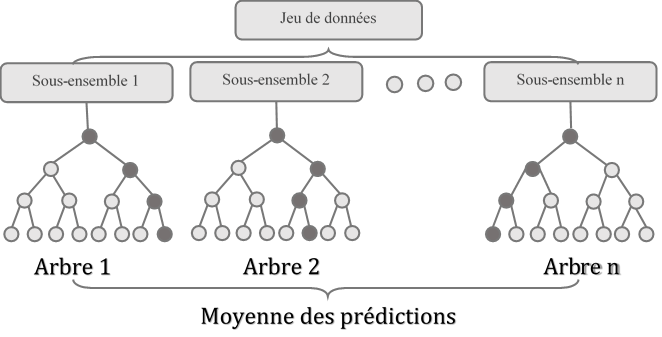
\includegraphics[width=\textwidth]{img/RFalgo.png}}
        \caption{ Random Forest Algorithme}
        \label{RF_algo}
\end{figure}
\begin{tcolorbox}
\footnotesize {
\begin{enumerate}
\item Des sous-ensembles aléatoires sont créés à partir du jeu de données d'origine (Bootstrapping\footnote{Bootstrap aggregating, est une technique d’échantillonnage permette de créer des sous-ensembles d’observations à partir du jeu de données d’origine, avec remplacement.}).
\item sur chaque nœud de l’arbre de décision, un seul ensemble aléatoire d’entités est pris en compte pour déterminer la meilleure répartition.
\item Un modèle d'arbre de décision est entraîné sur chacun des sous-ensembles.
\item La prédiction finale est calculée en faisant la moyenne des prédictions de tous les arbres de décision.
\end{enumerate}
}
\end{tcolorbox}

Cet algorithme a plusieurs hyperparamètres\footnote{hyperparamètre est un paramètre dont la valeur est définie avant le début du processus d'apprentissage.} qui peuvent mener au sur-apprentissage du modèle, ainsi qu'ils joue un rôle primordial dans l'apprentissage du modèle, ces paramètres sont:
\begin{itemize}
    \item[\textbullet] Le nombre d'arbres de régression;
    \item[\textbullet] La profondeur maximale d’un arbre;
    \item[\textbullet] Le nombre de variables d'entrée par noeud.
\end{itemize}



\subsection{Gradient Boosting Machine}
\textit{Gradient Boosting Machine} (GBM) \citep{friedman2002stochastic} est une technique d'apprentissage automatique des problèmes de régression et de classification, qui produit un modèle de prédiction sous la forme d'un ensemble de modèles de prédiction faibles, généralement des arbres de décision. L'idée de gradient boosting est née de l'observation de Leo Breiman en 1997, où il a considéré cette algorithme comme un outil d'optimisation sur une fonction de coût \citep{breiman1997arcing}, des algorithmes de gradient boosting de régression ont ensuite été développés en 2001 par Jerome H. Friedman \citep{friedman2001greedy}.\\

GBM utilise la technique de boosting\footnote{C'est un processus séquentiel dans lequel chaque modèle suivant tente de corriger les erreurs du modèle précédent.}, combinant plusieurs apprenants faibles (\textit{Weak learners}) pour former un apprenant fort (\textit{Strong learner}). Il est à noter que les arbres de régression sont utilisés comme apprenant de base (\textit{base learner}). Le principe de base est de construire une séquence de modèles de sorte que chaque étape, chaque modèle ajouté à la combinaison, apparaisse comme un pas vers une meilleure solution.\\


Cet algorithme suit les étapes suivantes:
\begin{enumerate}
\item Entraîner un simple régresseur linéaire ou un arbre de décision sur les données;
\item Calculer les résidus d'erreur (égale à la valeur cible réelle moins la valeur cible prédite)
$h_1(x)=y-f_1(x)$
\item Entraîner un nouveau modèle sur les résidus d'erreur en tant que variable cible avec les mêmes variables d'entrée $h_1(x)$;
\item Ajouter les résidus prédits aux prédictions précédentes, ce qui signifie la création d'un nouveau modèle, 
$f_2(x)=f_1(x)+h_1(x)$
\item Entraîner un autre modèle sur les résidus qui reste encore. C’est-à-dire $h_2(x)=y-f_2(x)$
\item Et répétez les étapes 2 à 5 jusqu'à ce qu'il commence le sur-apprentissage ou que la somme des résidus devienne constante. Le sur-apprentissage peut être contrôlé en vérifiant systématiquement la précision des données de validation.
$ f_m(x)=f_{(m-1)}(x)+ h_{(m-1)}(x)$ avec $h_{(m-1)}(x)=y- f_{(m-1)}(x)$
\end{enumerate}

\begin{tcolorbox}
\footnotesize {
\begin{enumerate}
\item Initialiser le résultat;
\item Itérer de 1 au nombre total des arbres;
	\begin{enumerate}
		\item Mettre à jour les pondérations pour les cibles en fonction de la série précédente (plus élevées pour celle mal classée);
		\item Ajuster le modèle sur un sous-échantillon de données sélectionné;
		\item Faire des prédictions sur l’ensemble des observations;
		\item Mettre à jour la sortie avec les résultats actuels en tenant compte du taux d’apprentissage;
	\end{enumerate}
\item Renvoyer la sortie finale.\\
\end{enumerate}
}
\end{tcolorbox}
À son tour GBM a quelques hyperparamètres qui requièrent l'optimisation afin d'éviter le sur-apprentissage, ces hyperparamètres sont:
\begin{itemize}
    \item[\textbullet] Le nombre d'arbres de régression;
    \item[\textbullet] La profondeur maximale d’un arbre;
    \item[\textbullet] Le nombre de variables d'entrée par noeud;
    \item[\textbullet] Le taux d'apprentissage lors de la construction du modèle.
\end{itemize}

%%%%%%%%%%%%%%%%%%%%%%%%%%%%%%%%%%%%%%%%%%%%%%%%%%%%%%%%%%%%%%%%%%%%%%%%%%%%%%%%%%%%%%%%%%%%%%%%%%%%%%%%%%%%%%%%%%%%%%%%%%%%%%%
\subsection{eXtreme Gradient Boosting : XGBoost}
\textit{XGBoost} (XGB) signifie \textit{eXtreme Gradient Boosting} est une implémentation open source populaire et efficace de l'algorithme gradient boosting trees, développé par Tianqi Chen\footnote{pour plus d'info: https://tqchen.github.io/} en 2016. \\

Comme nous avons déjà cité dans l'explication de l'algorithme précédent GBM, c'est un algorithme d'apprentissage supervisé qui tente de prédire avec précision une variable cible en combinant les estimations d’un ensemble de modèles plus simples et plus faibles. \\

En revanche, l'algorithme XGB est distingué par sa flexibilité et sa portabilité, en effet il fournit un \textit{Tree Boosting} parallélisé qui résout de nombreux problèmes de science de données d'une manière rapide et précise. Notamment, il a démontré son efficacité dans plusieurs compétitions d’apprentissage automatique, car il gère variété de types de données, de relations et de distributions, ainsi qu'un grand nombre de ses hyperparamètres pouvant être réglés et optimisés pour des améliorations au niveau d'apprentissage \citep{chen2016xgboost}.\\


Un estimateur $\phi $ additif à K arbre, de l'algorithme XGB, se formalise pour des entrées $(x_i, y_i)\in R^m\times R$ par l’équation \ref{eq1}.
\begin{equation}\label{eq1}
    \widetilde{y_l}=\phi (x_i)=\sum_{i=1}^{N}f_k(x_i), f_k \in \mathcal{F}
\end{equation}
Où $\widetilde{y_l}$ est l’estimation de $y_i$ et $\mathcal{F}= f(x) = \omega_{q(x)} (q:R^m \xrightarrow{}T, \omega \in R^T$ est l’espace des représentants des arbres de décisions et de régressions (CART). T et $\omega_i $ désignent respectivement le nombre de feuilles de l’arbre et la valeur associée aux points de la $i^{ème}$ feuille. $q$ désigne la fonction de structure de l’arbre qui a un échantillon $x_i$ associe l’indice de la feuille à laquelle il appartient. Afin d’obtenir les fonctions utilisés dans le modèle, on cherche à minimiser la fonction objectif régularisée $\mathcal{L}$ donnée par l’équation \ref{eq2}.
\begin{equation}\label{eq2}
    \mathcal{L}(\phi) = \sum_i l(\widetilde{y_l},y_i)+\sum_{k}\Omega(f_k)
\end{equation}

où $\Omega(f_k) = \gamma T +\lambda \| \omega \|_2 + \alpha \| \omega \|_1$\\

$l$ Désigne une fonction de perte convexe et différentiable. Cette minimisation se fait de manière
gloutonne en améliorant l’estimateur par l’ajout d’un arbre à chaque itération. A l’itération t, on cherche
à ajouter un nouvel arbre $f_t$ qui améliore les estimations des modèles, i.e. qui minimise la fonction
objectif $\mathcal{L}_t$ à l’instant t donnée par l’équation \ref{eq3}, où $\widetilde{y}_{l}^{t-1}$ est l’estimation de $y_i$ à l’issue de l’itération
précédente.
\begin{equation}\label{eq3}
    \mathcal{L}_t = \sum_{i} l(y_i , \widetilde{y}_{l}^{t-1}) + f_{t}(x_i) + \Omega (f_t)
\end{equation}\\

En utilisant une approximation au deuxième ordre de $\mathcal{L}_t$et en éliminant les termes constants, on obtient la nouvelle fonction objectif $\widetilde{\mathcal{L}_t}$ donnée par l’équation \ref{eq4}.
\begin{equation}\label{eq4}
    \widetilde{\mathcal{L}_t} = \sum_{i}[g_{i}f_{t}(x_{i} + \frac{1}{2} h_{i}f_{t}^2(x_i)] + \Omega (f_t)
\end{equation}

où $ g_i = \partial_{\widetilde{y}_{l}^{t-1}} l(y_{i}, \widetilde{y}_{l}^{t-1}) $ et $ h_i = \partial_{\widetilde{y}_{l}^{t-1}}^2 l(y_{i}, \widetilde{y}_{l}^{t-1}) $\\

En plus du terme de régularisation $\Omega$ plusieurs autres outils permettent d’empêcher l’occurrence de surapprentissage.
Parmi ces derniers nous avons considérés dans notre étude les suivants :
\begin{itemize}
    \item [\textbullet] La profondeur maximale d’un arbre ;
    \item [\textbullet] Un facteur de rétrécissement $\eta$ appliqué aux poids w des arbres les plus récents ;
    \item [\textbullet] Un sous-échantillonnage aléatoire des colonnes au niveau de chaque arbre ;
    \item [\textbullet] Taux de la réduction des écarts.\\
\end{itemize}

Les trois algorithmes décrits précédemment (RF, GBM, XGB) sont de famille ensembliste, ils sont basés principalement sur les arbres de régression, ces méthodes font générer plusieurs arbres qui sont ensuite combinées pour produire une prédiction finale. En effet, la combinaison d'un grand nombre d'arbres peut souvent entraîner des améliorations considérables sur la précision et la performance des prévisions.\\

Par ailleurs, la quatrième algorithme de cette étude est \textit{Deep learning} qui se base particulièrement sur des neurones artificielles. Dans ce qui suit nous détaillons ce genre d'algorithme.  
%%%%%%%%%%%%%%%%%%%%%%%%%%%%%%%%%%%%%%%%%%%%%%%%%%%%%%%%%%%%%%%%%%%%%%%%%%%%%%%%%%%%%%%%%%%%%%%%%%%%%%%%%%%%%%%%%%%%%
\subsection{Réseau de Neurone Artificiel}
L’\textit{Intelligence Artificielle}, branche de l’Informatique fondamentale s’est
développée avec pour objectif la simulation des comportements du cerveau
humain. Les premières tentatives de modélisation du cerveau sont anciennes
et précèdent même l’ère informatique. C’est en 1943 que Mc Culloch (neuro-
physiologiste) et Pitts (logicien) ont proposé les premières notions de \textit{neurone
formel}. Ce concept fut ensuite mis en réseau avec une couche d’entrée et une
sortie par Rosenblatt en 1959 pour simuler le fonctionnement rétinien et tacher
de reconnaître des formes. C’est l’origine du \textit{perceptron}. Cette approche dite 
\textit{connexioniste} a atteint ses limites technologiques, compte tenu de la puissance 
de calcul de l’époque, mais aussi théoriques au début des années 70.\\

Au début des années 80 ont permis de relancer l’approche connexioniste. Celle-
ci a connu au début des années 90 un développement considérable si l’on
considère le nombre de publications et de congrès qui lui ont été consacrés
mais aussi les domaines d’applications très divers où elle apparaît. Ainsi, 
les réseaux de neurones connaissent un regain d’intérêt et même un énorme battage médiatique sous l’appellation d’apprentissage profond (\textit{deep learning}).\\

Les réseaux de neurones artificiels consistent en des modèles plus ou moins
inspirés du fonctionnement cérébral de l’être humain en se basant principalement
sur le concept de neurone biologique (Cf. Fig. \ref{neuron_bio}), qui se compose de :
noyau\footnote{intègre les signaux entrants et génère un signal sortant vers axone}, 
axone\footnote{transmet des signaux électriques aux dendrites d'une autre cellule à l'aide de synapses
}, 
dendrites et 
synapse\footnote{recueillir des signaux électriques.}. Les neurones sont faits pour transmettre des informations.\\

\begin{figure}[!htb]
        \center{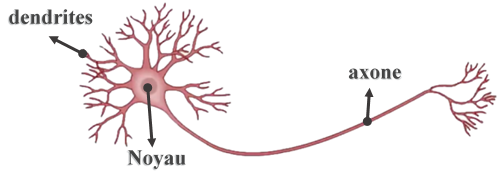
\includegraphics[width=10cm]{img/neuronbio.png}}
        \caption{ Neurone Biologique}
        \label{neuron_bio}
\end{figure}


Un neurone artificiel ou un perceptron en termes simples, calcule une « somme pondérée » de son entrée, ajoute un biais et décide ensuite s’il doit être faire une telle action ou non (Cf. Fig. \ref{neuron_art}).
Par exemple un neurone $$y=\sum(poids*entrées)+biais$$

\begin{figure}[!htb]
        \center{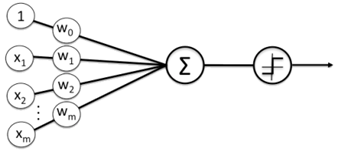
\includegraphics[width=10cm]{img/neuronartif.png}}
        \caption{Neurone Artificiel}
        \label{neuron_art}
\end{figure}

\subsubsection{Fonctions d’activation}\label{fun_activ}
Les fonctions d'activation prennent comme paramètres la somme pondérée des entrées ainsi que le seuil d’activation. Elle calcule la valeur de sortie à partir du résultat de la fonction de combinaison : $S_j=f(v_j)$ avec $S_j$ est la valeur de sortie, $f$ est la fonction d’activation, et $v_j$ est la fonction de transition.

\paragraph*{Fonction à seuil « Step function »}
\begin{wrapfigure}{r}{0.2\textwidth}
    \vspace{-1 cm}
    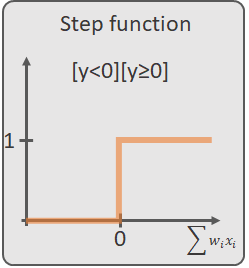
\includegraphics[width=0.2\textwidth]{img/stepfunc.png}
    \vspace{-1 cm}
\end{wrapfigure}
C’est une fonction d’activation basée sur un seuil. Si la valeur de $y$ dépasse une certaine valeur, le neurone est activé. L’inconvénient de ce type des fonctions est qu'elles ne prennent pas des valeurs intermédiaires. Cependant, elles fonctionnent parfaitement pour les problèmes qui ont des sorties binaires. 


\paragraph*{Fonction Linéaire}
\begin{wrapfigure}{r}{0.2\textwidth}
    \vspace{-1 cm}
    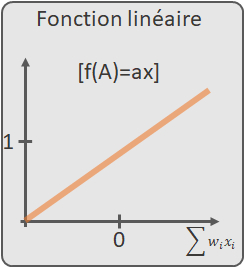
\includegraphics[width=0.2\textwidth]{img/linfunc.png}
    \vspace{-1 cm}
\end{wrapfigure}
C’est une fonction en ligne droite où l'activation est proportionnelle à l'entrée (qui est la somme pondérée du neurone). 
De cette façon, cela donne une gamme d'activations qui n'est pas forcément binaire comme dans le cas précédant de \textit{step function}.
L'inconvénient de cette fonction est que la dérivée est une constante. Peu importe le nombre de couches dont nous disposons, si toutes sont de nature linéaire, la fonction d'activation finale de la dernière couche n'est rien d'autre qu'une fonction linéaire de l'entrée de la première couche ! Cela signifie que ces couches peuvent être remplacées par une seule couche. Alors nous avons besoin d’une fonction qui nous donne la possibilité d'empiler des couches.


\paragraph*{Fonction sigmoïde}
\begin{wrapfigure}{r}{0.2\textwidth}
    \vspace{-1 cm}
    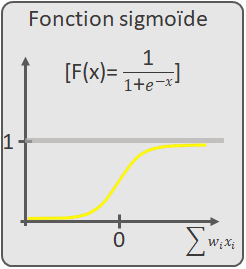
\includegraphics[width=0.2\textwidth]{img/segfunc.png}
    \vspace{-1 cm}
\end{wrapfigure}
C’est une fonction de nature non linéaire qui permet d'empiler des couches. Ainsi, elle donnera une activation analogique contrairement à la fonction à seuil. Il est à noter que toute modification mineure des valeurs de X dans cette région au voisinage de 0 entraînera une modification significative des valeurs de Y. Ce qui distingue cette fonction est que, contrairement à la fonction linéaire, la sortie de la fonction d'activation sera toujours dans la plage (0,1) par rapport à ($-\infty, \infty$) de la fonction linéaire. La fonction sigmoïde est l’une des fonctions d’activation les plus utilisées. 

\paragraph*{Fonction tanh}
\begin{wrapfigure}{r}{0.2\textwidth}
    \vspace{-1 cm}
    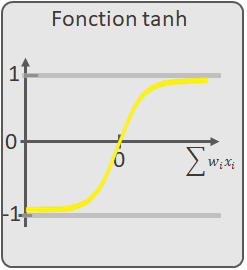
\includegraphics[width=0.2\textwidth]{img/tanhfunc.png}
    \vspace{-1 cm}
\end{wrapfigure}
Cette fonction ressemble à la fonction Sigmoïde. La différence avec la fonction Sigmoïde est que la fonction Tanh produit un résultat compris entre -1 et 1. La fonction Tanh est en terme général préférable à la fonction Sigmoïde car elle est centrée sur zéro. Les grandes entrées négatives tendent vers -1 et les grandes entrées positives tendent vers 1. Mis à part cet avantage, la fonction Tanh possède les mêmes autres inconvénients que la fonction Sigmoïde.

\paragraph*{Fonction ReLu « rectified linear unit »}
\begin{wrapfigure}{r}{0.2\textwidth}
    \vspace{-1 cm}
    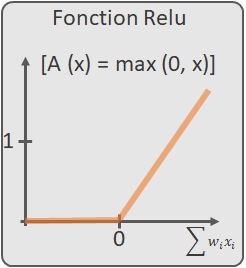
\includegraphics[width=0.2\textwidth]{img/relufunc.png}
\end{wrapfigure}
Pour résoudre le problème de saturation des deux fonctions précédentes (Sigmoïde et Tanh) il existe la fonction ReLU (Unité de Rectification Linéaire). Cette fonction est la plus utilisée. La fonction ReLU est interprétée par la formule: $f(x) = max(0, x)$. Si l'entrée est négative la sortie est 0 et si elle est négative alors la sortie est x. Cette fonction d'activation augmente considérablement la convergence du réseau et ne sature pas.
Mais la fonction ReLU n'est pas parfaite. Si la valeur d'entrée est négative, le neurone reste inactif, ainsi les poids ne sont pas mis à jour et le réseau n’apprend pas. ReLu est de nature non linéaire, cela signifie qu'elle nous donne la possibilité d'empiler des couches. La plage de ReLu est [0, $\infty$).


\subsubsection{Perceptron Multicouche MLP}
Le Perceptron Multicouche (MLP) est un des réseaux de neurones les plus utilisés pour des problèmes d’approximation, de classification et de prédiction. Il est habituellement constitué de trois ou plusieurs couches de neurones totalement connectées : une couche d’entrées, une de sortie et une ou plusieurs couches cachées.\\ 

Dans le cas général, un Perceptron multicouche peut posséder un nombre de couches quelconque et un nombre de neurones par couche également quelconque \citep{parizeau2004perceptron}. La taille (définie par le nombre de nœuds dans chaque couche cachée) optimale du réseau dépend de la complexité du problème et l’architecture choisie. Ce type de réseau fait partie de la famille des réseaux non bouclés (Feedforward network), c’est-à-dire qu’en mode normal d’utilisation, l’information se propage dans un sens unique, des entrées vers les sorties sans aucune rétroaction.\\

La figure \ref{MLP_fig} explicite l’exemple d’un réseau contenant une couche d’entrée, deux couches cachées et une couche de sortie. La couche d’entrée représente une couche virtuelle associée aux entrées du système, elle est composée de 3 paramètres et elle ne contient pas de neurone. Par contre, on distingue 3 neurones dans la première couche cachée, 4 neurones dans la deuxième et 2 neurones dans la couche de sortie. Les sorties des neurones
de la dernière couche correspondent aux sorties du réseau.

\begin{figure}[!htb]
        \center{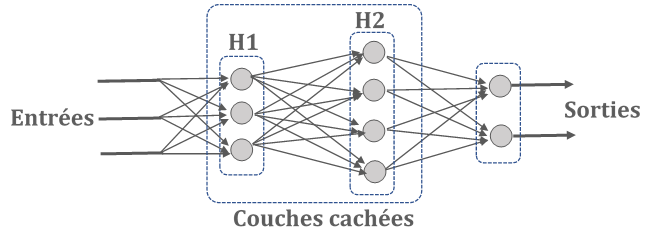
\includegraphics[width=\linewidth]{img/mlp.png}}
        \caption{Schéma d'un perceptron multicouche}
        \label{MLP_fig}
\end{figure}

\subsubsection{Apprentissage du MLP}

L’apprentissage du réseau de neurones a pour finalité que ce réseau donne les bonnes sorties sur un ensemble d’exemples, appelé \textit{ensemble de test}. Pour cela, on va utiliser un ensemble d’exemples sur lequel le réseau va s’entraîner et apprendre. Cet ensemble s’appelle l’\textit{ensemble d’apprentissage}. Les exemples de l’ensemble de test n’appartiennent pas à l’ensemble d’apprentissage. Ainsi, avec cette méthode basée sur la distinction entre l’ensemble d’apprentissage et celui du test, le réseau de neurones doit être capable de généralisation. Dans la plupart des architectures, l’apprentissage se traduit par un changement dans la valeur des poids qui relient les neurones d’une couche à l’autre.\\

Dans notre étude, nous avons utilisé un apprentissage de type \textit{supervisé} qui a pour principe d’ajuster les poids à la base de la comparaison des sorties connues aux sorties prévues par le réseau de telle façon que l’écart entre les deux soit minimal. Par conséquent, trouver les poids optimums pour le réseau de neurones est équivaut à la recherche du minimum global de la fonction coût $E$. Un ensemble de règles bien définies permettant de réaliser un tel processus d’adaptation des poids constitue ce qu’on appelle l’\textit{algorithme d’apprentissage du réseau} et l'approche adoptée au cours de ce travail est la \textit{rétro-propagation}.\\

En fait, la rétro-propagation permet la recherche d’un minimum local de la fonction d’erreur $E$ à travers la mise à jour des poids du réseau. Cette mise à jour se fait par plusieurs méthodes, la plus utilisée étant la descente du gradient (traduction libre de Gradient descent), elle consiste à retrancher le gradient de la fonction d’erreur multiplié par un taux fixe de la valeur du poids de l’itération qui précède. Le taux $\eta$ étant de sens opposé par rapport au gradient de la fonction d’erreur \citep{gunther2010neuralnet}.

Ainsi, les poids sont ajustés par la règle suivante :
            \begin{equation}
            \Delta\omega_{ij}^{(t)}=\omega_{ij}^{(t+1)}-\omega_{ij}^{(t)}=-\eta
            \frac{\partial E^{(t)}}{\partial \omega_{ij}^{(t)}}
            \end{equation}
            où $t$ est l'indice de l'itération.\\

Afin de rendre l'apprentissage plus stable, un \emph{moment} est ajouté à la formule précédente traduisant l'influence du poids de l'itération précédente :
            \begin{equation}
            \Delta\omega_{ij}^{(t)}= -\omega_{ij}^{(t)}=-\eta \frac{\partial
            E^{(t)}}{\partial \omega_{ij}^{(t)}} + \mu \Delta\omega_{ij}^{(t-1)}
            \end{equation}

%%%%%%%%%%%%%%%%%%%%%%%%%%%%%%%%%%%%%%%%%%%%%%%%%%%%%%%%%%%%%%%%%%%%%%%%%%%%%%%%%%%%%%%%%%%%%%%%%%%
\section{Configurations expérimentales}\label{config}
%%%%%%%%%%%%%%%%%%%%%%%%%%%%%%%%%%%%%%%%%%%%%%%%%%%%%%%%%%%%%%%%%%%%%%%%%%%%%%%%%%%%%%%%%%%%%%%%%%%
\subsection{Par plateforme et par algorithme}\label{config_pl_algo}
L'objectif principal de notre étude est d'évaluer la sensibilité de la performance des modèles développés à la plateforme et l'algorithme utilisés dans le cas d'un problème de régression, et qui traite l'estimation de la visibilité horizontale à partir des sorties d'un modèle de prévision numérique du temps. Pour atteindre cet objectif, nous avons effectué plusieurs configurations expérimentales combinant les plateformes open source (\textit{Scikit-learn}, \textit{H2O}, \textit{WEKA}, \textit{Tensorflow} et \textit{Keras}) et les algorithmes d'apprentissage automatique adoptés (Random Forest, Gradient Boosting Machine, eXtreme Gradient Boosting et Deep Learning).\\

Dans la première phase de modélisation, les modèles ont été développé à la base des configurations par défaut implémenté dans chaque algorithme et chaque plateforme. Autrement dit, les hyperparamètres de la configuration de base ont été utilisés. Dans la suite, on résumera ces paramètres par algorithme pour chaque plateforme.\\


\begin{itemize}
    \item[\ding{233}]\textbf{Random Forest}\\%%%%%%%%%%%%%%%%%%%%%%%%%%%%%%%%%%%%%%%%%%%%%%%%%%%%%%%%%%%%%%%%%%%%%%%%%%%%%%%%%%%%%
    
    Le tableau  \ref{tab:RF} récapitule les principaux hyperparamètres adoptés pour l'algorithme \textit{Random Forest} pour les plateformes retenues. Il est à noter que l'appellation des hyperparamètres diffèrent d'une plateforme à une autre. Ceci a constitué un challenge pour la mise en place de notre étude. Certains paramètres sont décrits brièvement comme note de bas du tableau. Il est à noter que cet algorithme a été utilisé sur trois plateformes : \textit{Scikit-learn}, \textit{H2O} et \textit{WEKA}.\\
\\
\\

        \begin{table}[h!]
        \centering
        \begin{threeparttable}[t]
        \begin{tabular}{|c||p{8cm}p{2cm}|}
        \hline
        plateforme & \multicolumn{2}{|c|}{Valeur des hyperparamètres}  \\ \hline
        \multirow{6}{*}{Scikit-learn} 
        & n\_estimators & 10  \\
        & min\_samples\_split & 2  \\ 
        & min\_samples\_leaf & 1 \\
        & max\_features & auto\tnote{1}\\
        & max\_depth & None\tnote{2}\\
        & bootstrap & True\tnote{3}\\
         \hline
        \multirow{4}{*}{H2O} 
        & ntrees & 50  \\
        & max\_depth & 20\\
        & min\_rows & 1  \\ 
        & mtries & -1\tnote{4}\\
         \hline
        \multirow{3}{*}{WEKA} 
        & numEtirations & 100  \\
        & maxDepth & 0\\
        & numFeatures & 0  \\ 
         \hline
        \end{tabular}
        \footnotesize{
        \begin{tablenotes}
              \item[1] max\_features=n\_features; 
              \item[2] nœuds sont développés jusqu'à ce que toutes les feuilles soient pures ou jusqu'à ce que toutes les feuilles contiennent moins de min\_samples\_split;
              \item[3]si False, le jeu de données est utilisé complètement pour construire chaque arbre;
              \item[4]le nombre de variable est p / 3 pour la régression (où p est le nombre de prédicteurs).
        \end{tablenotes}
        }
       \end{threeparttable}
        \caption{Les hyperparamètres de RF choisis par défaut pour chaque plateforme}
        \label{tab:RF}
        \end{table}

    \item[\ding{233}]\textbf{Gradient Boosting Machine}\\%%%%%%%%%%%%%%%%%%%%%%%%%%%%%%%%%%%%%%%%%%%%%%%%%%%%%%%%%%%%%%%%%%%%%%%%%
    
    Le tableau  \ref{tab:GBM} récapitule les principaux hyperparamètres adoptés pour l'algorithme \textit{Gradient Boosting Machine} pour les plateformes retenues : \textit{Scikit-learn} et \textit{H2O}.\\
        \begin{table}[h!]
        \centering
        \begin{tabular}{|c||p{8cm}p{2cm}|}
        \hline
        plateforme & \multicolumn{2}{|c|}{Valeur des hyperparamètres}  \\ \hline
        \multirow{6}{*}{Scikit-learn} 
        & n\_estimators & 100  \\
        & min\_samples\_split & 2  \\ 
        & min\_samples\_leaf & 1 \\
        & max\_features & None\\
        & max\_depth & 3\\
        & learning\_rate  & 0.1\\
         \hline
        \multirow{4}{*}{H2O} 
        & ntrees & 50  \\
        & max\_depth & 5\\
        & min\_rows & 10  \\ 
        & learn\_rate & 0.1 \\
        & sample\_rate & 1 \\
         \hline
        \end{tabular}
        \caption{Les hyperparamètres de GBM choisis par défaut pour chaque plateforme}
        \label{tab:GBM}
        \end{table}
        
    \item[\ding{233}]\textbf{eXtreme Gradient Boosting}\\%%%%%%%%%%%%%%%%%%%%%%%%%%%%%%%%%%%%%%%%%%%%%%%%%%%%%%%%%%%%%%%%%%%%%%%%%%
        Le tableau  \ref{tab:GBM} récapitule les principaux hyperparamètres adoptés pour l'algorithme \textit{eXtreme Gradient Boosting} pour les plateformes retenues : \textit{Scikit-learn} et \textit{H2O}.\\
        \begin{table}[h!]
        \centering
        \begin{tabular}{|c||p{8cm}p{2cm}|}
        \hline
        plateforme & \multicolumn{2}{|c|}{Valeur des hyperparamètres}  \\ \hline
        \multirow{5}{*}{Scikit-learn} 
        & n\_estimators & 100  \\
        & gamma & 0 \\ 
        & colsample\_bytree & 3 \\
        & learning\_rate & 0.1\\
        & max\_depth & 3\\
         \hline
        \multirow{3}{*}{H2O} 
        & ntrees &   50 \\
        & max\_depth & 6\\
        & min\_rows &  1 \\ 
         \hline
        \end{tabular}
        \caption{Les hyperparamètres de XGB choisis par défaut pour chaque plateforme}
        \label{tab:XGB}
        \end{table}

    \item[\ding{233}]\textbf{Deep Learning}\\%%%%%%%%%%%%%%%%%%%%%%%%%%%%%%%%%%%%%%%%%%%%%%%%%%%%%%%%%%%%%%%%%%%%%%%%%%%%%%%%%%%%%
Le tableau  \ref{tab:DL} récapitule les principaux hyperparamètres adoptés pour l'algorithme Deep Learning pour les plateformes retenues : \textit{Scikit-learn}, \textit{H2O}, \textit{WEKA} et \textit{Keras}.

        \begin{table}[h!]
        \centering
        \begin{threeparttable}[t]
        \begin{tabular}{|c||p{8cm}p{1.5cm}|}
        \hline
        plateforme & \multicolumn{2}{|c|}{Valeur des hyperparamètres}  \\ \hline
        \multirow{4}{*}{Scikit-learn} 
        & activation & relu  \\
        & hidden\_layer\_sizes & 100  \\
        & max\_iter & 200 \\
        & num hidden layer & 1 \\
         \hline
        \multirow{3}{*}{H2O} 
        & activation & Rec\\
        & size hidden layers & 200  \\
        & num hidden layers & 2  \\ 
         \hline
        \multirow{3}{*}{WEKA} 
        & hidden\_layer & a\tnote{1}  \\
        & learning\_rate & 0.3 \\
        & momentum & 0.2  \\ 
         \hline
        \multirow{3}{*}{KERAS} 
        &Cet outil n'a pas de configuration par défaut pour le deep learning. Pour spécifier un perceptron simple, il faut ajouter une couche qui relie directement la couche d’entrée (nombre de neurones = nombre de variables prédictives) avec la couche de sortie, tout en précisant une fonction d’activation.&\\
         \hline
        \end{tabular}
        \footnotesize{
            \begin{tablenotes}
                  \item[1]  a= (attributs + classes) / 2, i= attributs, o= classes , t= attributs + classes."
            \end{tablenotes}
        }
        \end{threeparttable}
        \caption{Les hyperparamètres de DL choisis par défaut pour chaque plateforme}
        \label{tab:DL}
        \end{table}
        
\end{itemize}





\newpage

\subsection{Optimisation des hyperparamètres}\label{opt_algo}
Vu que les algorithmes utilisés dans cette étude ont un nombre très important des hyperparamètres, alors leur optimisation est nécessaire car elle nous aide à trouver le modèle optimal minimisant une fonction de perte prédéfinie sur des données de test.\\

Dans ce travail nous avons utilisé 2 approches d'optimisation des hyperparamètres:\\
\begin{itemize}
    \item [\ding{109}] \textbf{Grid search:}\\ 
    
    C'est une méthode d’optimisation (hyperparameter optimization) qui va nous permettre de tester une série de paramètres et de comparer les performances pour en déduire le meilleur paramétrage. Ainsi, pour chaque paramètre, on détermine un ensemble de valeurs que l’on souhaite tester. Par exemple, dans le cas d’un Random Forest on pourrait tester :
    \begin{itemize}
        \item[\textbullet] Nombre d’arbres : \{ 10, 20, 30 \}
        \item[\textbullet] Nombre de variables sélectionnées : \{ 2, 3, 4, 5 \}\\
    \end{itemize}
    
Le Grid Search croise simplement chacune de ces hypothèses et va créer un modèle pour chaque combinaison de paramètres. Dans notre exemple nous aurons $3 \times 4 = 12$ modèles à construire. Grid Search a aussi ses limites puisque c’est l'utilisateur qui définit à l’avance les paramètres qu'il veut tester.\\ 
    \item [\ding{109}] \textbf{Random search:}\\ 
    
    C'est une technique dans laquelle des combinaisons aléatoires des hyperparamètres sont utilisées pour trouver la meilleure solution d'un modèle développé.\\
\end{itemize}

Ces approches d'optimisation sont utilisées par plateforme et par algorithme pour trouver le meilleur modèle. 

%%%%%%%%%%%%%%%%%%%%%%%%%%%%%%%%%%%%%%%%%%%%%%%%%%%%%%
\subsection{Analyse croisée par plateforme et par algorithme} \label{sec:ana-cross}
L'un des objectifs principaux de ce stage est d'évaluer la sensibilité de la performance du modèle développé à la plateforme open source et à l'algorithme Datamining choisis. Pour atteindre cet objectif, nous allons intégrer les hyperparamètres optimums obtenus soit par Grid search soit par Random search pour une plateforme donnée, dans le même algorithme mais pour une autre plateforme.\\

Par exemple si l'algorithme Random Forest dans la plateforme \textit{Scikit-learn} nous donne un erreur minimal avec un nombre d'arbres égale à 20, nous essayerons de faire appel au même algorithme (Random Forest) dans \textit{H2O} et \textit{WEKA} avec nombre d'arbre égale à 20, et d'évaluer l'impact sur la performance du modèle développé.\\

Tenant compte du fait que l'appellation des hyperparamètres diffèrent d'une plateforme à une autre, nous avons limité notre analyse croisée par plateforme et par algorithme, aux hyperparamètres dont les équivalents existent dans les deux plateformes comparées. Par exemple: l'hyperparamètre  \textbf{n\_estimators} qui indique le nombre d'arbre pour Random Forest en Scikit-learn, son équivalent en H2O est \textbf{ntrees} et dans \textit{WEKA} c'est \textbf{numEtirations}. Pour les autres hyperparamètres, ils ont gardé leurs valeurs par défaut. 


%%%%%%%%%%%%%%%%%%%%%%%%%%%%%%%%%%%%%%%%%%%%%%%%%%%%%%%%%%%%%%%%%%%%%%%%%%%%%%%%%%%%%%%%%%%%%%%%%%%
\section{Outils de Diagnostics }
%%%%%%%%%%%%%%%%%%%%%%%%%%%%%%%%%%%%%%%%%%%%%%%%%%%%%%%%%%%%%%%%%%%%%%%%%%%%%%%%%%%%%%%%%%%%%%%%%%%
Tenant compte de l'intérêt émergent à l'utilisation du Datamining dans pas mal de secteurs socio-économiques, le nombre d’outils d’exploration de données disponibles ne cesse de croître. Par conséquent, la concurrence entre les développeurs de logiciels d'exploration de données augmente également et le choix de l'outil le plus approprié devient de plus en plus difficile. Ainsi, la comparaison des outils d'exploration de données devient nécessaire même si elle n'est pas évidente. Au cours de cette section, nous allons expliciter certains critères de comparaison des plateformes retenues ainsi que les critères d'évaluation de la performance des algorithmes Datamining utilisés.

\subsection{Critères de comparaison des plateformes utilisées}
La comparaison entre plateformes open sources n'est pas évidente car elle fait appel à plusieurs critères (structures de données, les algorithmes implémentés, capacités de visualisation, langages de programmation, options d'importation et d'exportation, etc.). Pour ce faire, on s'est focalisé sur les critères suivants et qui ont été adoptés par \cite{chen2007survey} : les caractéristiques générales, la gestion des données, leur fonctionnalité et le mode d'utilisation.\\

\begin{itemize}
    \item[\ding{233}]\textbf{ Les caractéristiques générales :}\\
    Les caractéristiques générales considérées de la plateforme comprennent le nom de la plateforme, l'architecture, le système d’exploitation et le langage de programmation. En ce qui concerne l’architecture, les outils du Datamining peuvent être subdivisées en architecture autonome (standalone) et/ou architecture client /serveur. Le premier type ne nécessite aucun logiciel autre que le système d’exploitation, contrairement à l’architecture client / serveur. L'une des tendances émergentes est le nombre croissant d'interfaces Web fournissant l'exploration de données. Par conséquent, une architecture de service \textit{cloud} basée sur le Web sera également incluse en tant que valeur possible pour l'architecture des plateformes.\\
    
    \item[\ding{233}] \textbf{La gestion des données :}\\
    Tenant compte de la diversité des types de données, il est impossible de trouver un outil Datamining qui exploite toute sorte de format de données.
    Les outils du Datamining nécessite une intégration avec des systèmes de gestion de base de données (database systems) ou avec des entrepôts de données (data warehouse) pour la sélection des données, leur prétraitement et transformation, etc.\\ 
    
    Toutes les plateformes n’ont pas les mêmes caractéristiques de base de données en termes de modèle de données, taille possible des données, format des données et options d'importation. Ainsi, la comparaison portera sur les sources possibles de données (MS SQL SERVER \footnote{Microsoft SQL Server est un système de gestion de base de données}, MS EXCEL \footnote{Microsoft Excel est un logiciel tableur de la suite bureautique Microsoft Office.}, Oracle \footnote{un système de gestion de base de données relationnelle.}, PostgreSQL\footnote{un système de gestion de base de données relationnelle et objet.} ...), les connexions aux bases de données (JDBC \footnote{Java Data Base Connectivity}, ODBC \footnote{Open Database Connectivity},..).\\
    
    De plus, les formats de données possibles sont classés selon les formats suivants : ARFF (Attribute-Relation File Format), CSV (valeurs séparées par des virgules)\footnote{Comma-separated values} ou Excel. La dernière caractéristique importante pour la gestion des données est la taille de l'ensemble de données. Pour chaque outil Datamining, on spécifiera s'il convient à traiter un petit ou un grand volume de données (Big data).
    \\
    
    \item[\ding{233}] \textbf{La fonctionnalité:}\\
    Pour le critère de fonctionnalité, les outils Datamining seront comparés en ce qui concerne les méthodes / tâches offertes par les plateformes : prétraitement des données, régression, classification, regroupement et visualisation de modèle.
    \\
    
    \item[\ding{233}] \textbf{Le mode d'utilisation:}\\
    Le mode d'utilisation inclut l’existence d'une GUI (interface utilisateur graphique)\footnote{Graphical User Inerface} ou d'une CLI (interface en ligne de commande) \footnote{Command-line interface}. Pour les groupes d’utilisateurs, ils sont subdivisés en  application d’entreprise ou applications dans la recherche et de l'enseignement.\\
    
\end{itemize}
%%%%%%%%%%%%%%%%%%%%%%%%%%%%%%%%%%%%%%%%%%%%%%%%%%%%%%%
\subsection{Critères de comparaison des algorithme utilisées}\label{dig_algo_perf}
\begin{itemize}
\item[\ding{233}] \textbf{Évaluation de la performance des algorithmes développés}\\

L’évaluation de la performance des modèles développés fait l’objet de scores objectifs qui permettent de
suivre l’évolution de leur qualité. Ainsi, plusieurs scores se trouvent dans la littérature. La formulation des scores continus de vérification, utilisés dans cette étude, est comme suit:\\

\begin{itemize}
    \item[\ding{109}] L’\textit{erreur absolue moyenne} (MAE) représente la moyenne arithmétique de la valeur absolue des écarts de la valeur estimée (F) à l’observation (O).
    \begin{equation}
        MAE = \frac{1}{N} \sum_{i=1}^{N}\lvert F_{i}-O_{i} \rvert
    \end{equation}
    \item[\ding{109}]  L’\textit{erreur quadratique moyenne} (Root Mean Square Error, RMSE) mesure la dispersion des valeurs estimées par rapport à l’observation, et reflète ainsi la variabilité au sein de l’échantillon de données. Plus ce score est faible, plus la dispersion du modèle est faible.
    \begin{equation}
        RMSE = \left[ \frac{1}{N} \sum_{i=1}^{N} (F_{i}-O_{i})^2  \right]^{1/2}
    \end{equation}
    \item[\ding{109}] Le \textit{coefficient de corrélation} de Pearson CC mesurant la corrélation entre les prédictions du modèle et la variable à prédire.
    \begin{equation}
        CC = \frac{\sum_{i=1}^{N} (F_{i}-\Bar{F})(O_{i}-\Bar{O})}{\sqrt{\sum_{i=1}^{N} (F_{i}-\Bar{F})^2}\sqrt{\sum_{i=1}^{N} (O_{i}-\Bar{O})^2}}
    \end{equation}
    Où $\Bar{F}$ et $\Bar{O}$ sont les valeurs moyennes de la valeur estimée et de l'observation respectivement.
    \item[\ding{109}] Le \textit{biais} d'un estimateur est la moyenne de différence entre la valeur attendue de cet estimateur et la valeur réelle du paramètre estimé.
    \begin{equation}
        BIAIS = \frac{1}{N} \sum_{i=1}^{N}(F_{i}-O_{i})
    \end{equation}
    Ces scores sont utilisés pour quantifier la qualité d'estimation de la visibilité horizontale par les algorithmes développés dans le cadre de cette étude.\\
\end{itemize}

Les algorithmes décrits précédemment sont tous de type supervisé. Ainsi, les algorithmes basés sur des stratégies adaptatives
(boosting, gradient boosting) ou aléatoires (bagging, random forest) permettant d’améliorer l’ajustement par une combinaison
ou agrégation d’un grand nombre de modèles tout en évitant ou contrôlant le sur-ajustement. Ces algorithmes se base l'approche \textit{Biais-Variance Tradeoff} pour contrôler le sur-ajustement ou sur-apprentissage (overfitting).\\

\item[\ding{233}] \textbf{Vérification de sur-apprentissage: Biais-Variance Tradeoff}\\

    \begin{itemize}
        \item[\ding{109}] Le biais qui représente l’erreur provenant d’hypothèses erronées dans l’algorithme
        d’apprentissage. Ainsi, un biais élevé peut être lié à un algorithme qui manque de relations pertinentes entres les données d’entrée et les sorties prévues (sous-apprentissage).\\
        
        \item[\ding{109}] La variance qui représente l’erreur due à la sensibilité aux petites fluctuations de l’échantillon d’apprentissage. Ainsi, une variance élevée peut entraîner une sur-apprentissage, autrement dit modéliser le bruit aléatoire des données d’apprentissage plutôt que les sorties prévues.
            \begin{figure}[!htb]
            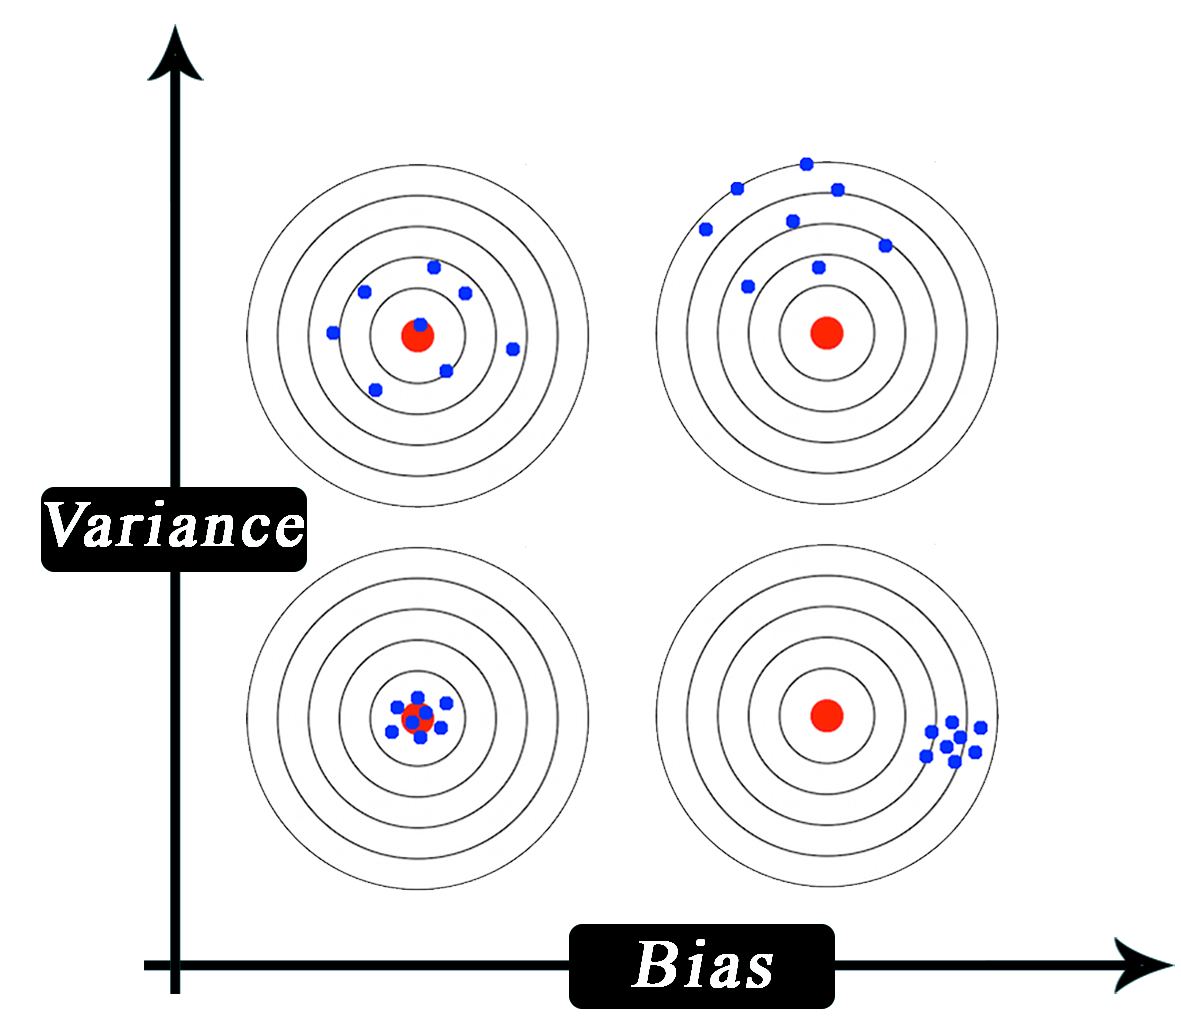
\includegraphics[width=7cm]{img/biasV.png}\hfill
            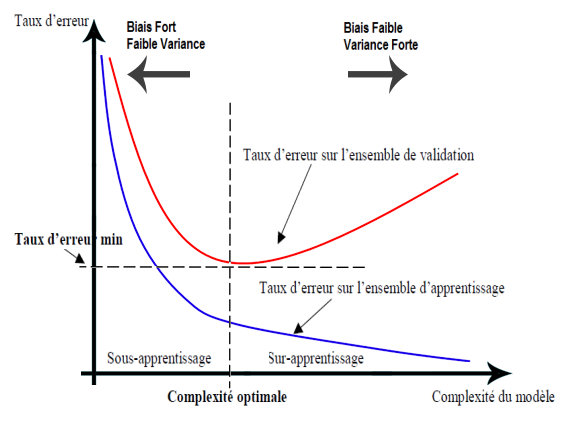
\includegraphics[width=9cm]{img/biasV3.png}
            \caption{Bias-Variance Tradeoff}\label{biasVar}
            \end{figure}
    \end{itemize}
\end{itemize}





